% vim: set spell spelllang=en tw=100 et sw=4 sts=4 foldmethod=marker foldmarker={{{,}}} :

\documentclass{beamer}

\usepackage{tikz}
\usepackage{xcolor}
\usepackage{complexity}
\usepackage{hyperref}
\usepackage{microtype}
\usepackage{amsmath}                   % \operatorname
\usepackage{amsfonts}                  % \mathcal
\usepackage{amssymb}                   % \nexists
\usepackage[vlined]{algorithm2e} % algorithms
\usepackage{centernot}
\usepackage{listings}
\usepackage{csquotes}
\usepackage{fancyvrb}

\RequirePackage[tt=false, type1=true]{libertine}
\RequirePackage[varqu]{zi4}
\RequirePackage[libertine]{newtxmath}
\RequirePackage[T1]{fontenc}

\newcommand*{\rom}[1]{\emph{\romannumeral #1 \relax}}

\usetikzlibrary{shapes, arrows, shadows, calc, positioning, fit}
\usetikzlibrary{decorations.pathreplacing, decorations.pathmorphing, shapes.misc}
\usetikzlibrary{tikzmark, backgrounds}
\usetikzlibrary{trees}

\tikzset{processarrow/.style={->, very thick, decorate, decoration={snake, post length=0.5mm}}}
\tikzset{brace/.style={decorate, decoration={brace}, very thick}}

\definecolor{uofguniversityblue}{rgb}{0, 0.219608, 0.396078}

\definecolor{uofgheather}{rgb}{0.356863, 0.32549, 0.490196}
\definecolor{uofgaquamarine}{rgb}{0.603922, 0.72549, 0.678431}
\definecolor{uofgslate}{rgb}{0.309804, 0.34902, 0.380392}
\definecolor{uofgrose}{rgb}{0.823529, 0.470588, 0.709804}
\definecolor{uofgmocha}{rgb}{0.709804, 0.564706, 0.47451}
\definecolor{uofgsandstone}{rgb}{0.321569, 0.278431, 0.231373}
\definecolor{uofgforest}{rgb}{0, 0.2, 0.129412}
\definecolor{uofglawn}{rgb}{0.517647, 0.741176, 0}
\definecolor{uofgcobalt}{rgb}{0, 0.615686, 0.92549}
\definecolor{uofgturquoise}{rgb}{0, 0.709804, 0.819608}
\definecolor{uofgsunshine}{rgb}{1.0, 0.862745, 0.211765}
\definecolor{uofgpumpkin}{rgb}{1.0, 0.72549, 0.282353}
\definecolor{uofgthistle}{rgb}{0.584314, 0.070588, 0.447059}
\definecolor{uofgrust}{rgb}{0.603922, 0.227451, 0.023529}
\definecolor{uofgburgundy}{rgb}{0.490196, 0.133333, 0.223529}
\definecolor{uofgpillarbox}{rgb}{0.701961, 0.047059, 0}
\definecolor{uofglavendar}{rgb}{0.356863, 0.301961, 0.580392}

% {{{ theme things
\useoutertheme[footline=authortitle]{miniframes}
\useinnertheme{rectangles}

\setbeamerfont{block title}{size={}}
\setbeamerfont{title}{size=\large,series=\bfseries}
\setbeamerfont{section title}{size=\large,series=\mdseries}
\setbeamerfont{author}{size=\normalsize,series=\mdseries}
\setbeamercolor*{structure}{fg=uofguniversityblue}
\setbeamercolor*{palette primary}{use=structure,fg=black,bg=white}
\setbeamercolor*{palette secondary}{use=structure,fg=white,bg=uofgcobalt}
\setbeamercolor*{palette tertiary}{use=structure,fg=white,bg=uofguniversityblue}
\setbeamercolor*{palette quaternary}{fg=white,bg=black}

\setbeamercolor*{titlelike}{parent=palette primary}

\beamertemplatenavigationsymbolsempty

\setbeamertemplate{title page}
{
    \begin{tikzpicture}[remember picture, overlay]
        \node at (current page.north west) {
            \begin{tikzpicture}[remember picture, overlay]
                \fill [fill=uofguniversityblue, anchor=north west] (0, 0) rectangle (\paperwidth, -3.0cm);
            \end{tikzpicture}
        };

        \node (logo) [anchor=north east, shift={(-2.2cm,-0.4cm)}] at (current page.north east) {
            
\includegraphics[keepaspectratio=true,scale=0.4]{UoG_keyline.pdf}
        };
        \node (logo2) [anchor=north, below = 0 of logo.south] {
            
\includegraphics[keepaspectratio=true,scale=0.025]{UStA_Logo_PR-REV.png}
        };
        \node (logo3) [anchor=west, right = 0 of $(logo2.east)!0.5!(logo.east)$] {
            
\includegraphics[keepaspectratio=true,scale=0.1]{kings.png}
        };

        \node [anchor=west, xshift=0.1cm, yshift=-0.6cm] at (current page.west |- logo.west) {
            \begin{minipage}{0.65\paperwidth}\raggedright
                {\usebeamerfont{title}\usebeamercolor[white]{}\inserttitle}\\[0.1cm]
                {\usebeamerfont{author}\usebeamercolor[white]{}\insertauthor}
            \end{minipage}
        };
    \end{tikzpicture}
}

\setbeamertemplate{section page}
{
    \begin{centering}
        \begin{beamercolorbox}[sep=12pt,center]{part title}
            \usebeamerfont{section title}\insertsection\par
        \end{beamercolorbox}
    \end{centering}
}

\newcommand{\frameofframes}{/}
\newcommand{\setframeofframes}[1]{\renewcommand{\frameofframes}{#1}}

\makeatletter
\setbeamertemplate{footline}
{%
    \begin{beamercolorbox}[colsep=1.5pt]{upper separation line foot}
    \end{beamercolorbox}
    \begin{beamercolorbox}[ht=2.5ex,dp=1.125ex,%
        leftskip=.3cm,rightskip=.3cm plus1fil]{author in head/foot}%
        \leavevmode{\usebeamerfont{author in head/foot}\insertshortauthor}%
        \hfill%
        {\usebeamerfont{institute in head/foot}\usebeamercolor[fg]{institute in head/foot}\insertshortinstitute}%
    \end{beamercolorbox}%
    \begin{beamercolorbox}[ht=2.5ex,dp=1.125ex,%
        leftskip=.3cm,rightskip=.3cm plus1fil]{title in head/foot}%
        {\usebeamerfont{title in head/foot}\insertshorttitle}%
        \hfill%
        {\usebeamerfont{frame number}\usebeamercolor[fg]{frame number}\insertframenumber~\frameofframes~\inserttotalframenumber}
    \end{beamercolorbox}%
    \begin{beamercolorbox}[colsep=1.5pt]{lower separation line foot}
    \end{beamercolorbox}
}

\makeatletter
\newenvironment{nearlyplainframe}[2][]{
    \def\beamer@entrycode{\vspace*{-\headheight}\vspace*{3pt}}
    \setbeamertemplate{headline}
    {%
        \begin{beamercolorbox}[colsep=1.5pt]{upper separation line head}
        \end{beamercolorbox}
        \begin{beamercolorbox}[ht=0.5ex,dp=0.125ex,%
            leftskip=.3cm,rightskip=.3cm plus1fil]{title in head/foot}%
        \end{beamercolorbox}%
        \begin{beamercolorbox}[ht=0.5ex,dp=0.125ex,%
            leftskip=.3cm,rightskip=.3cm plus1fil]{author in head/foot}%
        \end{beamercolorbox}%
        \begin{beamercolorbox}[colsep=1.5pt]{lower separation line head}
        \end{beamercolorbox}
        \vspace*{\headheight}
    }

    \setbeamertemplate{footline}
    {%
        \begin{beamercolorbox}[colsep=1.5pt]{upper separation line foot}
        \end{beamercolorbox}
        \begin{beamercolorbox}[ht=0.5ex,dp=0.125ex,%
            leftskip=.3cm,rightskip=.3cm plus1fil]{author in head/foot}%
        \end{beamercolorbox}%
        \begin{beamercolorbox}[ht=0.5ex,dp=0.125ex,%
            leftskip=.3cm,rightskip=.3cm plus1fil]{title in head/foot}%
        \end{beamercolorbox}%
        \begin{beamercolorbox}[colsep=1.5pt]{lower separation line foot}
        \end{beamercolorbox}
    }

    \begin{frame}[#1]{#2}
    }{
    \end{frame}
}
\makeatother

\makeatletter
\newenvironment{justborderframe}[2][]{
    \def\beamer@entrycode{\vspace*{-\headheight}}
    \setbeamertemplate{headline}
    {%
        \begin{beamercolorbox}[colsep=1.5pt]{upper separation line head}
        \end{beamercolorbox}
        \begin{beamercolorbox}[ht=0.5ex,dp=0.125ex,%
            leftskip=.3cm,rightskip=.3cm plus1fil]{title in head/foot}%
        \end{beamercolorbox}%
        \begin{beamercolorbox}[ht=0.5ex,dp=0.125ex,%
            leftskip=.3cm,rightskip=.3cm plus1fil]{author in head/foot}%
        \end{beamercolorbox}%
        \begin{beamercolorbox}[colsep=1.5pt]{lower separation line head}
        \end{beamercolorbox}
        \vspace*{\headheight}
    }

    \setbeamertemplate{footline}
    {%
        \begin{beamercolorbox}[colsep=1.5pt]{upper separation line foot}
        \end{beamercolorbox}
        \begin{beamercolorbox}[ht=0.5ex,dp=0.125ex,%
            leftskip=.3cm,rightskip=.3cm plus1fil]{author in head/foot}%
        \end{beamercolorbox}%
        \begin{beamercolorbox}[ht=0.5ex,dp=0.125ex,%
            leftskip=.3cm,rightskip=.3cm plus1fil]{title in head/foot}%
        \end{beamercolorbox}%
        \begin{beamercolorbox}[colsep=1.5pt]{lower separation line foot}
        \end{beamercolorbox}
    }

    \begin{frame}[#1]{}
    }{
    \end{frame}
}
\makeatother


% }}}

\author[\"Ozg\"ur Akg\"un \and Jessica Enright \and Christopher Jefferson \and \textbf{Ciaran
McCreesh} \and Patrick Prosser \and Steffen Zschaler]{
    \"Ozg\"ur Akg\"un \and Jessica Enright \and \\
    Christopher Jefferson \and Ciaran McCreesh \and \\
    Patrick Prosser \and Steffen Zschaler
}
\title[Finding Subgraphs With Side Constraints]{Finding Subgraphs \\With Side Constraints}

\begin{document}

{
    \usebackgroundtemplate{
        \tikz[overlay, remember picture]
        \node[at=(current page.south), anchor=south, inner sep=0pt]{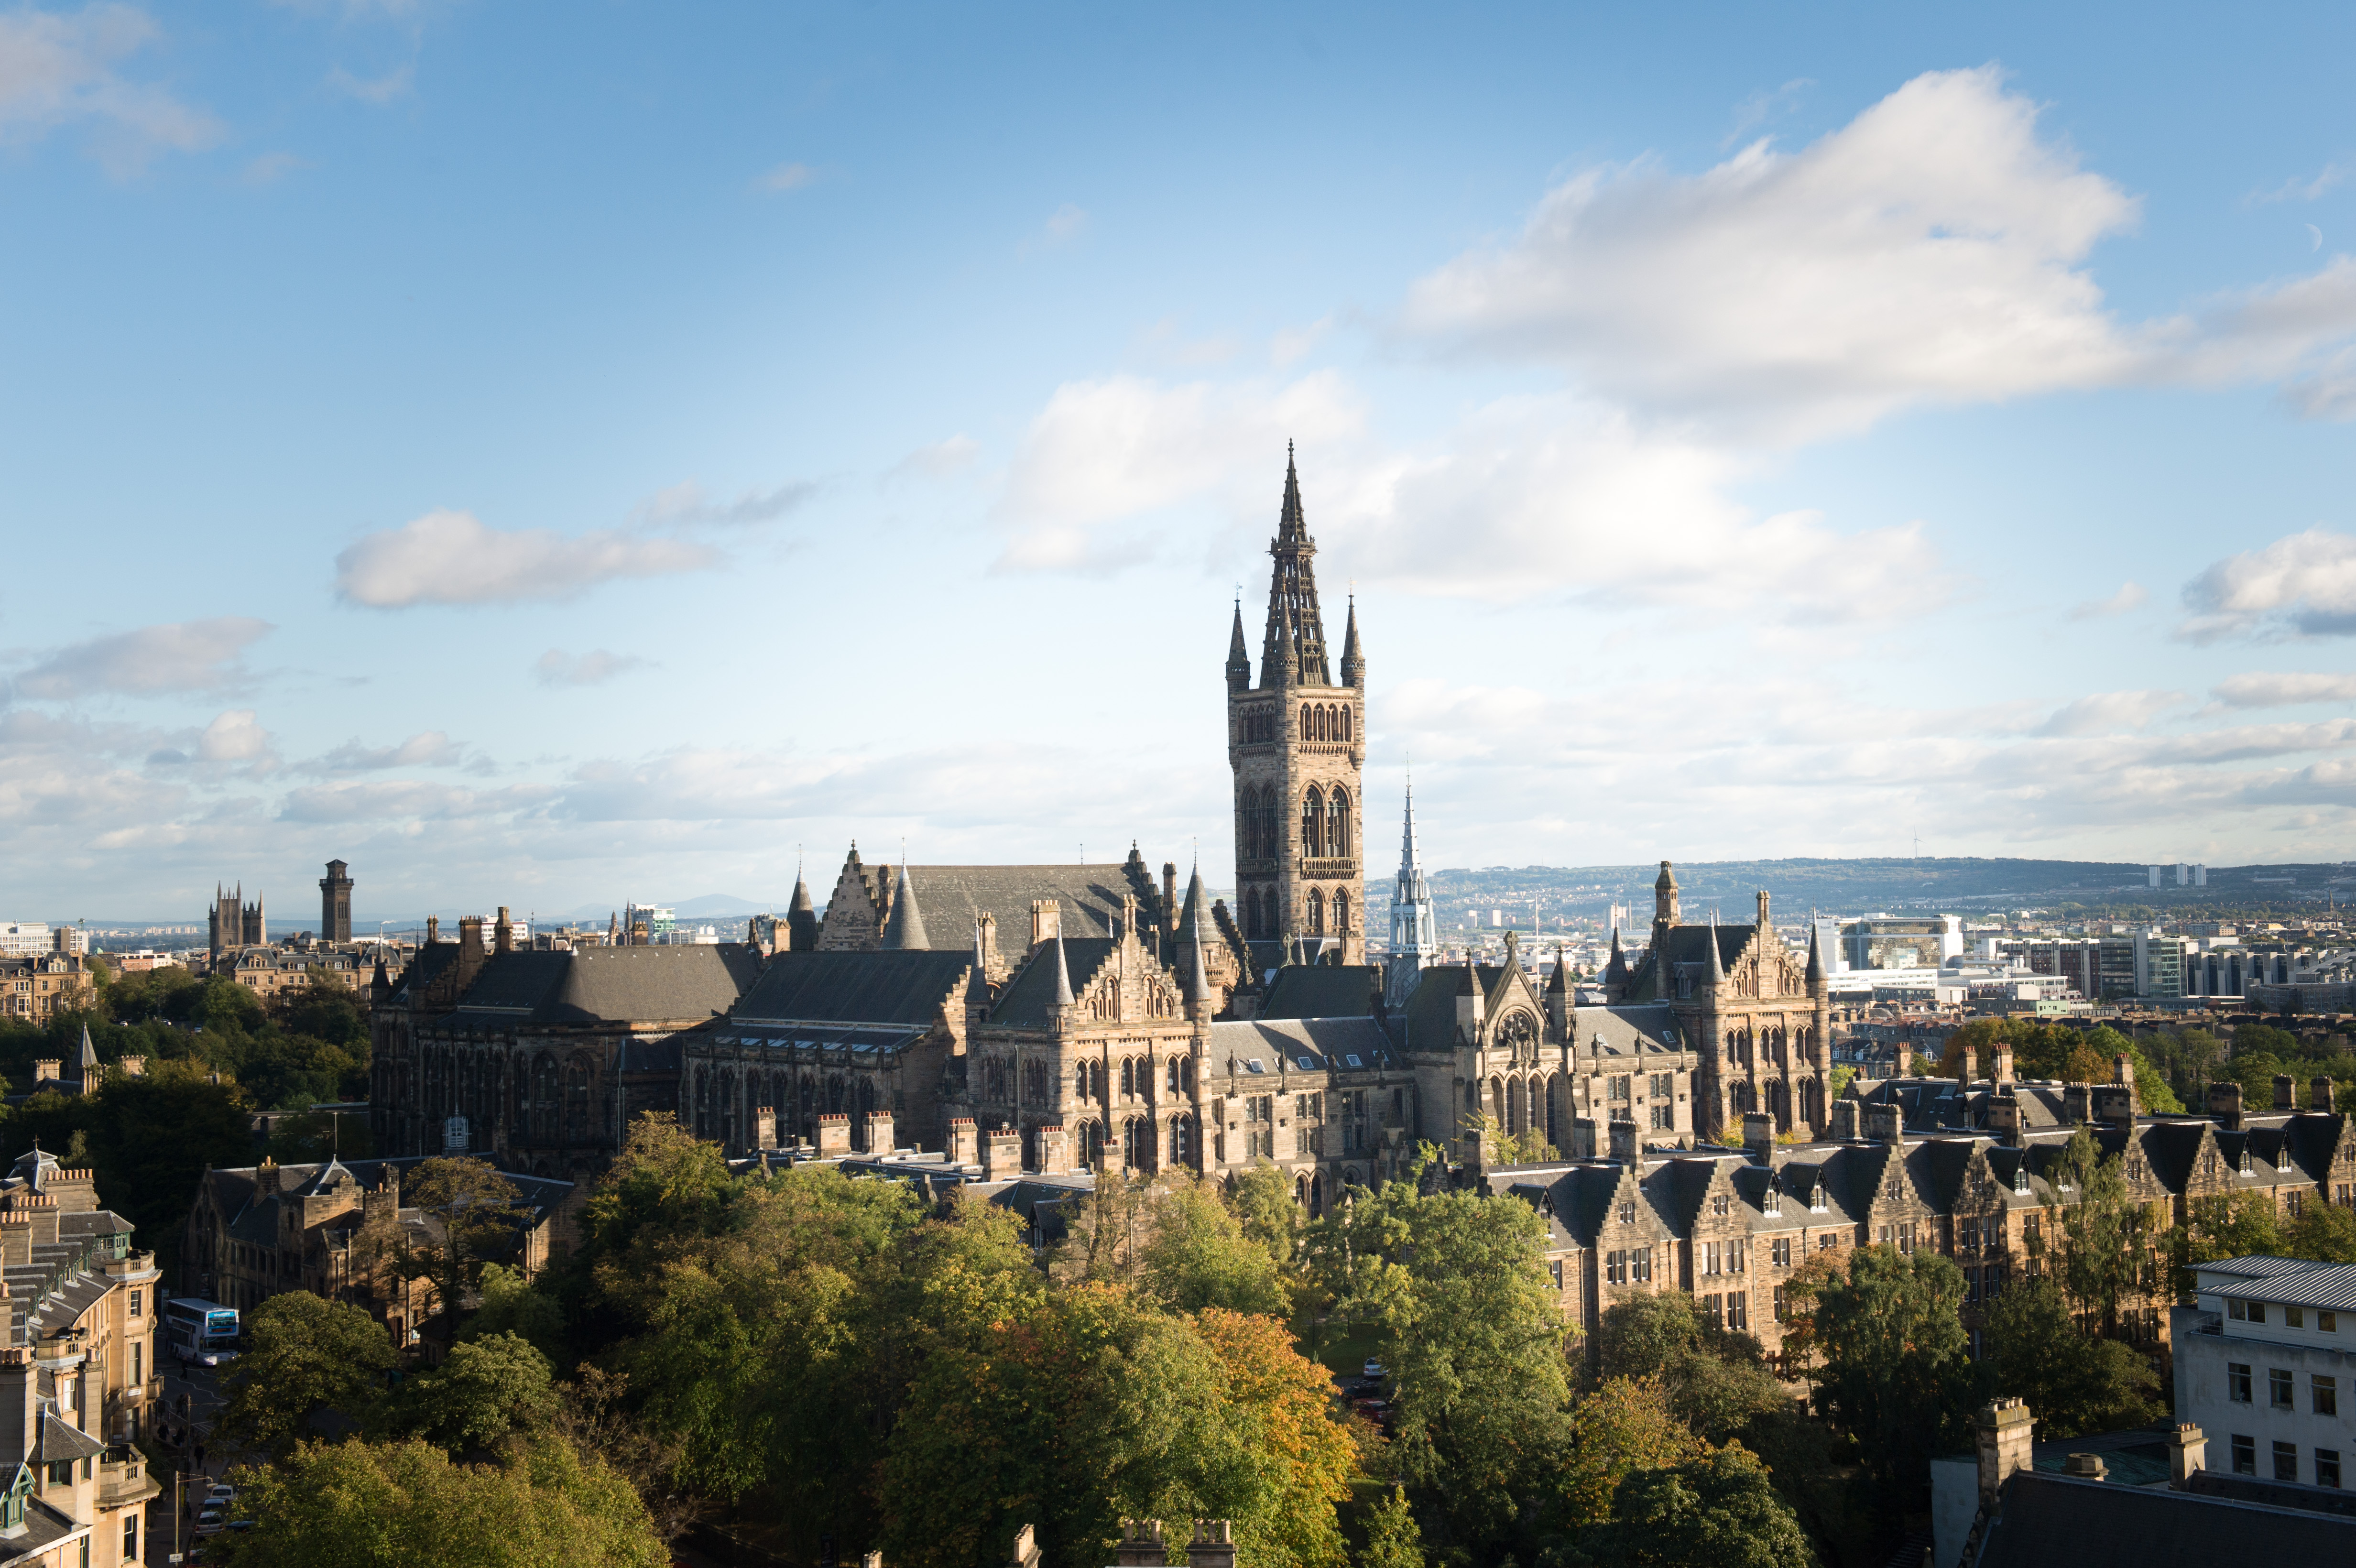
\includegraphics[keepaspectratio=true, height=\paperheight]{background.jpg}};
    }
    \begin{frame}[plain,noframenumbering]
        \titlepage
    \end{frame}
}

\begin{frame}{Modelling and Solving Subgraph Isomorphism}
    \begin{minipage}{0.25\paperwidth}
        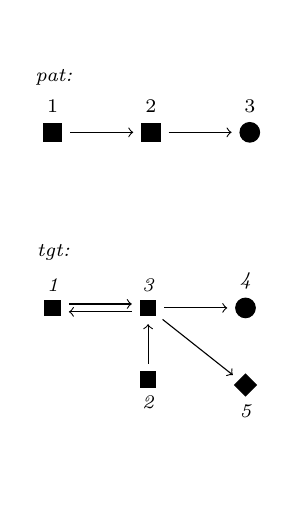
\begin{tikzpicture}
        \node [draw, fill] (P1) {}; \node [above=0cm of P1, font=\scriptsize] { 1 };
        \node [draw, fill, right=1cm of P1] (P2) {}; \node [above=0cm of P2, font=\scriptsize] { 2 };
        \node [draw, fill, circle, right=1cm of P2, inner sep=2.5pt] (P3) {}; \node [above=0cm of P3, font=\scriptsize] { 3 };
        \draw [->, shorten >=1mm, shorten <=1mm] (P1) -- (P2); node [midway, font=\scriptsize\itshape, above] { 1 };
        \draw [->, shorten >=1mm, shorten <=1mm] (P2) -- (P3); node [midway, font=\scriptsize\itshape, above] { 2 };
        \node [above=0.7cm of P1.west, anchor=west, xshift=-0.2cm] { pat: };

        \node [draw, fill, below=2cm of P1] (T1) {}; \node [above=0cm of T1, font=\scriptsize] { 1 };
        \node [draw, fill, right=1cm of T1] (T3) {}; \node [above=0cm of T3, font=\scriptsize] { 3 };
        \node [draw, fill, below=0.7cm of T3] (T2) {}; \node [below=0cm of T2, font=\scriptsize] { 2 };
        \node [draw, fill, circle, right=1cm of T3, inner sep=2.5pt] (T4) {}; \node [above=0cm of T4, font=\scriptsize] { 4 };
        \node [draw, fill, diamond, below=0.7cm of T4, inner sep=2pt] (T5) {}; \node [below=0cm of T5, font=\scriptsize] { 5 };
        \draw [->, shorten >=1mm, shorten <=1mm, transform canvas={yshift=0.5mm}] (T1) -- (T3); % node [midway, font=\scriptsize\itshape, above] { 2 };
        \draw [<-, shorten >=1mm, shorten <=1mm, transform canvas={yshift=-0.5mm}] (T1) -- (T3); % node [midway, font=\scriptsize\itshape, below] { 2 };
        \draw [->, shorten >=1mm, shorten <=1mm] (T2) -- (T3); % node [midway, font=\scriptsize\itshape, left] { 1 };
        \draw [->, shorten >=1mm, shorten <=1mm] (T3) -- (T4); % node [midway, font=\scriptsize\itshape, above] { 2 };
        \draw [->, shorten >=1mm, shorten <=1mm] (T3) -- (T5); % node [midway, font=\scriptsize\itshape, below] { 3 };
        \node [above=0.7cm of T1.west, anchor=west, xshift=-0.2cm] { tgt: };

        \node [above=1cm of P1] { ~ };
        \node [below=1cm of T2] { ~ };
            \end{tikzpicture}\end{minipage}\begin{minipage}[c]{0.1\paperwidth}~\end{minipage}\begin{minipage}[c]{0.6\paperwidth}
        \only<2>{\lstinputlisting[basicstyle=\scriptsize\ttfamily]{sip.essence}}%
        \only<3>{\lstinputlisting[basicstyle=\scriptsize\ttfamily]{sip-instance.essence}}%
        \only<4>{\lstinputlisting[basicstyle=\scriptsize\ttfamily]{sip-constraints.essence}}%
        \only<5>{\lstinputlisting[basicstyle=\scriptsize\ttfamily]{sip-solution.essence}}%
        \only<6>{\lstinputlisting[basicstyle=\scriptsize\ttfamily]{sip-induced.essence}}%
        \only<7>{\lstinputlisting[basicstyle=\scriptsize\ttfamily]{sip-induced-solution.essence}}%
    \end{minipage}
\end{frame}

\begin{frame}{Temporal Problems}
    \begin{minipage}{0.25\paperwidth}
        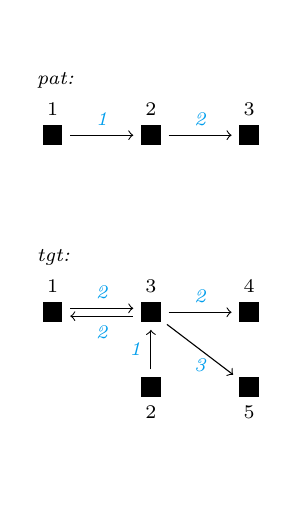
\begin{tikzpicture}
        \node [draw, fill] (P1) {}; \node [above=0cm of P1, font=\scriptsize] { 1 };
        \node [draw, fill, right=1cm of P1] (P2) {}; \node [above=0cm of P2, font=\scriptsize] { 2 };
        \node [draw, fill, right=1cm of P2] (P3) {}; \node [above=0cm of P3, font=\scriptsize] { 3 };
        \draw [->, shorten >=1mm, shorten <=1mm] (P1) -- (P2) node [midway, color=uofgcobalt, font=\scriptsize\itshape, above] { 1 };
        \draw [->, shorten >=1mm, shorten <=1mm] (P2) -- (P3) node [midway, color=uofgcobalt, font=\scriptsize\itshape, above] { 2 };
        \node [above=0.7cm of P1.west, anchor=west, xshift=-0.2cm, font=\scriptsize\itshape] { pat: };

        \node [draw, fill, below=2cm of P1] (T1) {}; \node [above=0cm of T1, font=\scriptsize] { 1 };
        \node [draw, fill, right=1cm of T1] (T3) {}; \node [above=0cm of T3, font=\scriptsize] { 3 };
        \node [draw, fill, below=0.7cm of T3] (T2) {}; \node [below=0cm of T2, font=\scriptsize] { 2 };
        \node [draw, fill, right=1cm of T3] (T4) {}; \node [above=0cm of T4, font=\scriptsize] { 4 };
        \node [draw, fill, below=0.7cm of T4] (T5) {}; \node [below=0cm of T5, font=\scriptsize] { 5 };
        \draw [->, shorten >=1mm, shorten <=1mm, transform canvas={yshift=0.5mm}] (T1) -- (T3) node [midway, color=uofgcobalt, font=\scriptsize\itshape, above] { 2 };
        \draw [<-, shorten >=1mm, shorten <=1mm, transform canvas={yshift=-0.5mm}] (T1) -- (T3) node [midway, color=uofgcobalt, font=\scriptsize\itshape, below] { 2 };
        \draw [->, shorten >=1mm, shorten <=1mm] (T2) -- (T3) node [midway, color=uofgcobalt, font=\scriptsize\itshape, left] { 1 };
        \draw [->, shorten >=1mm, shorten <=1mm] (T3) -- (T4) node [midway, color=uofgcobalt, font=\scriptsize\itshape, above] { 2 };
        \draw [->, shorten >=1mm, shorten <=1mm] (T3) -- (T5) node [midway, color=uofgcobalt, font=\scriptsize\itshape, below] { 3 };
        \node [above=0.7cm of T1.west, anchor=west, xshift=-0.2cm, font=\scriptsize\itshape] { tgt: };

        \node [above=1cm of P1] { ~ };
        \node [below=1cm of T2] { ~ };
            \end{tikzpicture}\end{minipage}\begin{minipage}[c]{0.1\paperwidth}~\end{minipage}\begin{minipage}[c]{0.6\paperwidth}
        \only<2>{\lstinputlisting[basicstyle=\scriptsize\ttfamily]{tsip-instance.essence}}%
        \only<3>{\lstinputlisting[basicstyle=\scriptsize\ttfamily]{tsip-exact-constraints.essence}}%
        \only<4>{\lstinputlisting[basicstyle=\scriptsize\ttfamily]{tsip-exact-solution.essence}}%
        \only<5>{\lstinputlisting[basicstyle=\scriptsize\ttfamily]{tsip-offset-constraints.essence}}%
        \only<6>{\lstinputlisting[basicstyle=\scriptsize\ttfamily]{tsip-offset-solution.essence}}%
        \only<7>{\lstinputlisting[basicstyle=\scriptsize\ttfamily]{tsip-embedding-constraints.essence}}%
        \only<8>{\lstinputlisting[basicstyle=\scriptsize\ttfamily]{tsip-embedding-solution.essence}}%
    \end{minipage}
\end{frame}

\begin{frame}{Retyping Problems}
    \begin{minipage}{0.25\paperwidth}
    \centering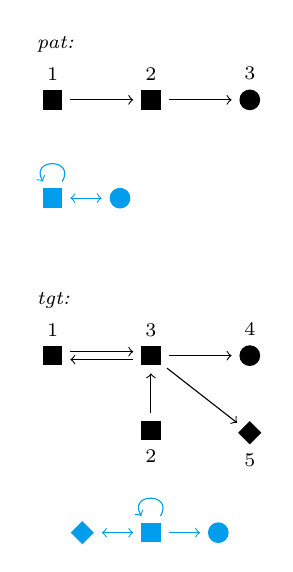
\begin{tikzpicture}
        \node [draw, fill] (P1) {}; \node [above=0cm of P1, font=\scriptsize] { 1 };
        \node [draw, fill, right=1cm of P1] (P2) {}; \node [above=0cm of P2, font=\scriptsize] { 2 };
        \node [draw, fill, circle, right=1cm of P2, inner sep=2.5pt] (P3) {}; \node [above=0cm of P3, font=\scriptsize] { 3 };
        \draw [->, shorten >=1mm, shorten <=1mm] (P1) -- (P2);
        \draw [->, shorten >=1mm, shorten <=1mm] (P2) -- (P3);
        \node [above=0.7cm of P1.west, anchor=west, xshift=-0.2cm, font=\scriptsize\itshape] { pat: };

        \begin{scope}[color=uofgcobalt]
        \node [draw, fill, below=1cm of P1] (PT1) {};
        \node [draw, fill, circle, inner sep=2.5pt, right=0.6cm of PT1] (PT2) {};
        \draw [<->, shorten >=1mm, shorten <=1mm] (PT1) -- (PT2);
        \draw [->, shorten >=1mm, shorten <=1mm] (PT1) to [out=60, in=120, looseness=8] (PT1);
        \end{scope}

        \node [draw, fill, below=3cm of P1] (T1) {}; \node [above=0cm of T1, font=\scriptsize] { 1 };
        \node [draw, fill, right=1cm of T1] (T3) {}; \node [above=0cm of T3, font=\scriptsize] { 3 };
        \node [draw, fill, below=0.7cm of T3] (T2) {}; \node [below=0cm of T2, font=\scriptsize] { 2 };
        \node [draw, fill, circle, right=1cm of T3, inner sep=2.5pt] (T4) {}; \node [above=0cm of T4, font=\scriptsize] { 4 };
        \node [draw, fill, diamond, below=0.7cm of T4, inner sep=2pt] (T5) {}; \node [below=0cm of T5, font=\scriptsize] { 5 };
        \draw [->, shorten >=1mm, shorten <=1mm, transform canvas={yshift=0.5mm}] (T1) -- (T3);
        \draw [<-, shorten >=1mm, shorten <=1mm, transform canvas={yshift=-0.5mm}] (T1) -- (T3);
        \draw [->, shorten >=1mm, shorten <=1mm] (T2) -- (T3);
        \draw [->, shorten >=1mm, shorten <=1mm] (T3) -- (T4);
        \draw [->, shorten >=1mm, shorten <=1mm] (T3) -- (T5);
        \node [above=0.7cm of T1.west, anchor=west, xshift=-0.2cm, font=\scriptsize\itshape] { tgt: };

        \begin{scope}[color=uofgcobalt]
        \node [draw, fill, below=2cm of T3] (TT1) {};
        \node [draw, fill, circle, inner sep=2.5pt, right=0.6cm of TT1] (TT2) {};
        \node [draw, fill, diamond, inner sep=2pt, left=0.6cm of TT1] (TT3) {};
        \draw [->, shorten >=1mm, shorten <=1mm] (TT1) -- (TT2);
        \draw [<->, shorten >=1mm, shorten <=1mm] (TT1) -- (TT3);
        \draw [->, shorten >=1mm, shorten <=1mm] (TT1) to [out=60, in=120, looseness=8] (TT1);
        \end{scope}
        \end{tikzpicture}\end{minipage}\begin{minipage}[c]{0.1\paperwidth}~\end{minipage}\begin{minipage}[c]{0.6\paperwidth}
        \only<2>{\lstinputlisting[basicstyle=\scriptsize\ttfamily]{retype-model.essence}}%
        \only<3>{\lstinputlisting[basicstyle=\scriptsize\ttfamily]{retype-constraints.essence}}%
        \only<4>{\lstinputlisting[basicstyle=\scriptsize\ttfamily]{retype-instance.essence}}%
        \only<5>{\lstinputlisting[basicstyle=\scriptsize\ttfamily]{retype-solutions.essence}}%
    \end{minipage}
\end{frame}

\begin{frame}{Costed Subgraph Isomorphism}
    \begin{itemize}
        \item We can look for the ``least expensive'' assignment:
    \lstinputlisting[basicstyle=\scriptsize\ttfamily]{costing.essence}
        \item Or something fancier like a Pareto front, or involving combinations of assignments.
    \end{itemize}
\end{frame}

\begin{frame}{Unfortunately\ldots}
    \only<1>{\centering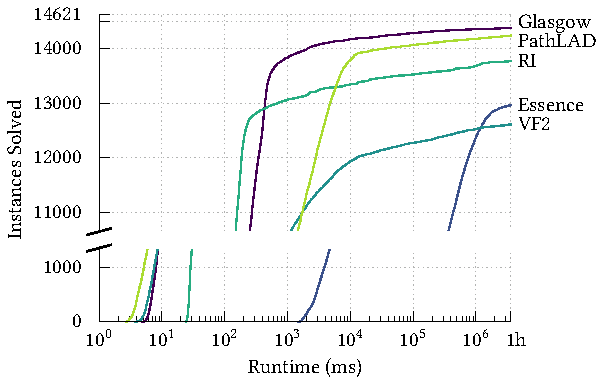
\includegraphics{gen-graph-glasgow-versus-minion-cumulative.pdf}}%
    \only<2>{\centering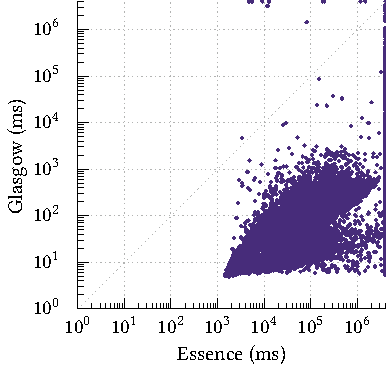
\includegraphics{gen-graph-glasgow-versus-minion-scatter.pdf}}
\end{frame}

\begin{frame}{Communicating Solvers}
    \begin{itemize}
        \item The Glasgow Subgraph Solver is basically a constraint programming solver for graph problems.
            \begin{itemize}
                \item Special data structures and propagation algorithms.
                \item Would be a lot of work to add all the usual general purpose constraints.
                \item Not particularly easy to add arbitrary other variables.
            \end{itemize}
        \item Idea: use a general CP solver to handle side constraints and additional variables.
    \end{itemize}
\end{frame}

\begin{frame}{How to Communicate?}
    \begin{itemize}
        \item External CP solver has a model of everything except (possibly) the graph constraints.
        \item Glasgow solver feeds partial assignments and can ask:
            \begin{itemize}
                \item Propagate, and either tell me ``unsatisfiable'', or list any deletions inferred.
                \item Give me one or all solutions respecting this assignment.
            \end{itemize}
        \item Simple text protocol, communicate over named pipes.
            \begin{itemize}
                \item Implemented in Minion, but nothing particularly solver-specific.
            \end{itemize}
    \end{itemize}
\end{frame}

\begin{frame}{High Level Modelling and Coordination}
    \begin{itemize}
        \item Main challenges are:
            \begin{itemize}
                \item We need the two solvers to have a consistent view of the graph variables.
                \item Recognising what the graph part of the problem is.
            \end{itemize}
        \item Essence toolchain is good at pattern matching.
        \item Minimal text file explaining variable remapping to the Glasgow solver.
    \end{itemize}
\end{frame}

\begin{frame}{When to Communicate?}
    \begin{itemize}
        \item Just check solutions?
        \item Propagate at the root node as well?
        \item Propagate at every node?
        \item Something cleverer?
    \end{itemize}
\end{frame}

\begin{frame}{Four Challenging Problems}
    \only<1>{\centering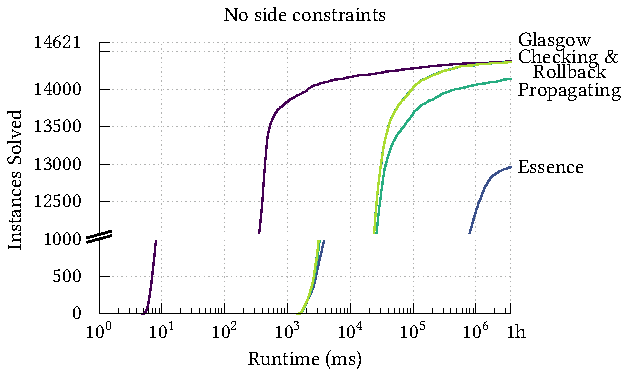
\includegraphics{gen-graph-nosideconstraints.pdf}}%
    \only<2>{\centering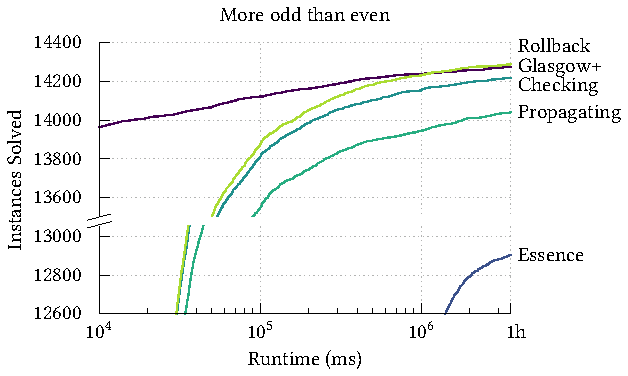
\includegraphics{gen-graph-oddeven.pdf}}%
    \only<3>{\centering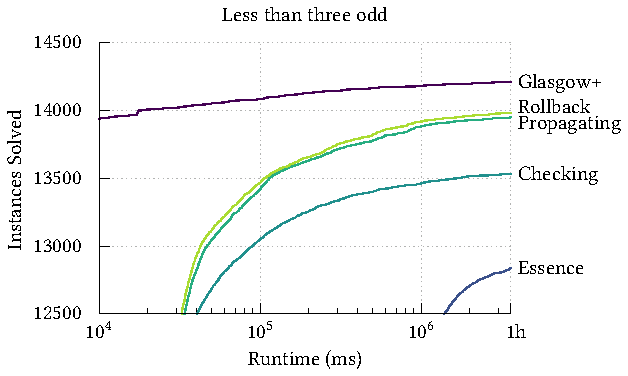
\includegraphics{gen-graph-mostlyodd.pdf}}%
    \only<4>{\centering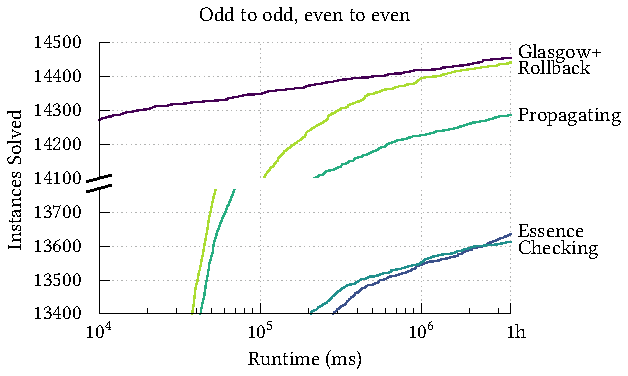
\includegraphics{gen-graph-parity.pdf}}%
\end{frame}

\begin{frame}{Rollback Communication}
    \begin{itemize}
        \item Propagate at the root node.
        \item Check solutions. If a solution is rejected:
            \begin{itemize}
                \item Backtrack and propagate.
                \item If this is rejected, backtrack and propagate again until success.
                \item Otherwise, continue without propagating.
            \end{itemize}
        \item Heavily inspired by backjumping, conflict analysis, and SMT, but doesn't require the CP
            solver to be able to produce conflict clauses.
    \end{itemize}
\end{frame}

\begin{frame}{Perspectives}
    \begin{itemize}
        \item For hard instances, this is great.
        \item Also extremely useful for prototyping and rapid data exploration.
        \item Very large startup overheads make this challenging for some other applications.
            \begin{itemize}
                \item But this is down to high level modelling rather than using a CP solver.
                \item Also questions about deployability\ldots
            \end{itemize}
        \item As is often the case, knowing when to do strong reasoning is critical.
    \end{itemize}
\end{frame}

{
    \usebackgroundtemplate{
        \tikz[overlay, remember picture]
        \node[at=(current page.south), anchor=south, inner
        sep=0pt]{\includegraphics[keepaspectratio=true, width=\paperwidth]{background2.jpg}};
    }

    \begin{frame}[plain,noframenumbering]
        \begin{tikzpicture}[remember picture, overlay]
            \node at (current page.north west) {
                \begin{tikzpicture}[remember picture, overlay]
                    \fill [fill=uofguniversityblue, anchor=north west] (0, 0) rectangle (\paperwidth, -2.6cm);
                \end{tikzpicture}
            };

        \node (logo) [anchor=north east, shift={(-2.2cm,-0.4cm)}] at (current page.north east) {
            
\includegraphics[keepaspectratio=true,scale=0.4]{UoG_keyline.pdf}
        };
        \node (logo2) [anchor=north, below = 0 of logo.south] {
            
\includegraphics[keepaspectratio=true,scale=0.025]{UStA_Logo_PR-REV.png}
        };
        \node (logo3) [anchor=west, right = 0 of $(logo2.east)!0.5!(logo.east)$] {
            
\includegraphics[keepaspectratio=true,scale=0.1]{kings.png}
        };

            \node [anchor=north west, shift={(0.6cm,-0.8cm)}] at (current page.north west) {
                \textcolor{white}{\url{https://ciaranm.github.io/}}
            };

            \node [anchor=north west, shift={(0.6cm,-1.4cm)}] at (current page.north west) {
                    \textcolor{white}{\href{mailto:ciaran.mccreesh@glasgow.ac.uk}{\nolinkurl{ciaran.mccreesh@glasgow.ac.uk}}}
            };
        \end{tikzpicture}
    \end{frame}
}

\end{document}

